\documentclass{VUMIFPSkursinis}
\usepackage{algorithmicx}
\usepackage{algorithm}
\usepackage{algpseudocode}
\usepackage{amsfonts}
\usepackage{amsmath}
\usepackage{bm}
\usepackage{caption}
\usepackage{color}
\usepackage{float}
\usepackage{graphicx}
\usepackage{listings}
\usepackage{subfig}
\usepackage{wrapfig}
\usepackage{lithuanian}
\usepackage{longtable}

\usepackage{enumitem}
%PAKEISTA, tarpai tarp sąrašo elementų
\setitemize{noitemsep,topsep=0pt,parsep=0pt,partopsep=0pt}
\setenumerate{noitemsep,topsep=0pt,parsep=0pt,partopsep=0pt}

% Titulinio aprašas
\university{Vilniaus universitetas}
\faculty{Matematikos ir informatikos fakultetas}
\department{Programų sistemų katedra}
\papertype{Kursinis darbas}
\title{Labai panašių neuroninių klasių atskyrimas dirbtiniais neuroniniais tinklais}
\titleineng{(Separation of very similar neuronal classes by artificial neural networks)}
\status{3 kurso 5 grupės studentai}
\author{Miglė Vaitulevičiūtė}
\supervisor{dr. Vytautas Valaitis}
\date{Vilnius – \the\year}

% Nustatymai
% \setmainfont{Palemonas}   % Pakeisti teksto šriftą į Palemonas (turi būti įdiegtas sistemoje)
%\bibliography{bibliografija}
\documentclass{article}
\usepackage[backend=biber]{biblatex}
\addbibresource{bibliografija.bib}
\begin{document}
	
% PAKEISTA	
\maketitle
\cleardoublepage\pagenumbering{arabic}
\setcounter{page}{2}

%TURINYS
\tableofcontents

\sectionnonum{Įvadas}

Darbo tikslas: patikrinti mokymosi tikslumo kokybę su skirtinų gylių dirbtiniais neuroniniais tinklais, kai mokymui yra naudojamas mažas paveikslėlių rinkinys.

Užduotys:
\begin{enumerate}
\item Pasirinkti analizuojamą dirbtinį neuroninį tinklą.
\item Pritaikyti ir modifikuoti neuronį tinklą išsikeltam darbo tikslui.
\item Gautą neuronį tinklą su skirtingais gyliais apmokyti.
\item Surasti ir naudoti geriausią optimizavimo funkciją.
\end{enumerate}


\section{Dirbtinis neuroninis tinklas}
Pagal apibendrintą žmogaus smegenų veikimą buvo sugalvoti dirbtiniai neuroniniai tinklai \cite{Goodfellow-et-al-2016}. Bendrai žmogaus smegenys turi šimtus
milijardų neuronų, kurie yra sujungti sinapsėsmis. Per tuos neuronus sklinda elektroniniai impulsai perduodantys informaciją - taip žmonės gali 
atpažinti objektus, garsus ir t.t. Dirbtiniai neuroniniai tinklai veikia panašiai. Jie irgi turi daug besijungiančių neuronų, kurie gauna informaciją ir 
pagal tą informaciją gali nuspręsti koks objektas yra paveikslėlyje. Tačiau ties tuo ir baigiasi žmogaus smegenų ir dirbtinių neuroninių tinklų panašumas, 
kadangi dirbtiniai neuroniniai tinklai yra kompiuterinė simuliacija - matematinis algoritmas su aritmetiniais kintamaisiais. Ši simuliacija yra suvokiama 
tik žmogui, kuris suprogramavo dirbtinį neuroninį tinklą, pačiam tinklui simuliacija nieko nereiškia, nuovokos nesuteikia.

\subsection{Dirbtinio neuroninio tinklo sudėtis}
Dirbtinis neuroninis tinklas yra sluoksnių rinkinys (1 pav.) - neuronų grupė sudaro sluoksnį, kuris yra sujungtas tarpusavyje su kitais sluoksniais. Vienas iš
sluoksnių privalo būti įvesties sluoksnis, kuris atitinkamai pagal užduoti gali gauti įvairios formos informaciją - paveiksliukai, vaizdo
medžiaga, garsas ir t.t. Ši informacija yra reikalinga tam, kad tinklas galėtų ją išanalizuoti ir išmokti. Tuo tikslu, kad vėliau gavęs panašią
informaciją galėtų ją atpažinti - tam reikalingas išeities sluoksnis. Jis yra priešingame dirbtinio neuroninio tinklo gale negu įeities sluoksnis.
Tarp anksčiau apibūdintų sluoksnių yra įvairaus dydžio sluoksnių sistema, kuri atlieka pagrindinį darbą \cite{Woodford-2018}.

\begin{figure}[h]
\centering
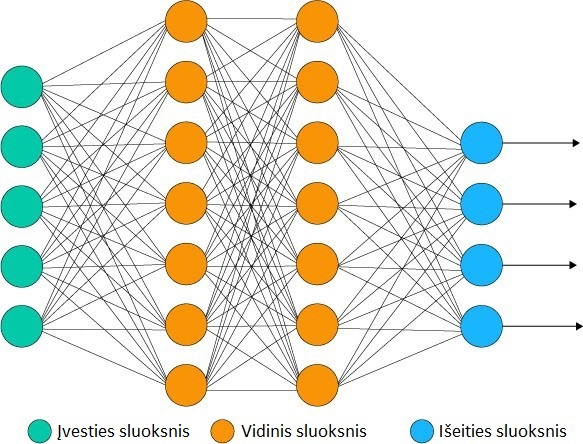
\includegraphics[width=0.5\textwidth]{img/NTSluoksniuSistema.jpeg}
\caption{Sluoksnių rinkinys}
\end{figure}

\subsection{Dirbtinio neuroninio tinklo veikimas}
Jungtys tarp neuronų yra pateiktos skaitine išraiška ir vadinamos svoriu. Kuo didesnis šis svoris tuo didesnę įtaką turi vienas neuronas kitam.
Vienam neuronui yra pateikiama visų prieš jį buvusių neuronų informacija ir jungčių svoriai. Kiekvieno neurono informacija yra sudauginama su
jo svoriu ir visi šie duomenys yra sudedami tarpusavyje. Taip iš vektoriaus gaunamas vienas rezultatas ir jei šis rezultatas tinka aktyvavimo
funkcijai, jis yra perduodamas tolimesniems neuronams. Tokio tipo veikimo dizainas yra vadinamas ,,feedforward'' tinklu.

Tačiau jungčių svoriai nėra pastovūs. Kai dirbtinis neuroninis tinklas mokosi, galutinis rezultatas yra lyginamas su tikėtinu teisingu rezultatu, jei šie
rezultatai skiriasi, svoriai yra keičiami atitinkamai, tai vadinama ,,backpropagation''. Tokiu būdu yra gerinamas rezultatas ir mažinamas skirtumas
tarp tikėtino ir gauto atsakymų.

\subsection{Aktyvavimo funkcijos}
Aktyvavimo funkcijų yra įvairių, kadangi sprendžiant tam tikrą problemą yra geriau naudoti vienas funkcijas, o kitas problemas - kitas funkcijas.
Pagrinde yra dviejų tipų aktyvavimo funkcijos - tiesinės ir netiesinės. Tiesinės nėra tokios populiarios, kadangi jos neleidžia įvesčiai
būti lanksčiai. Nors tiesinė funkcija labai dažnai naudojama išeities sluoksnyje.
Netiesinės funkcijos dažniausiai naudojamos vidiniuose sluoksniuose. Šiuo metu labiausiai naudojama yra ReLU, kadangi naudojant šią funkciją mokymo
rezultatai nuolatos gerėja, tačiau ReLU funkcijos spraustumas nesuteikia efektyvumo tinklui \cite{DBLP:journals/corr/XuWCL15}.

Aktyvavimo funkcijos yra skirstomos į:
\begin{itemize}
\item Tiesinė: 
\begin{itemize}
\item Žingsninė (binarinė) - išėjimas yra 0 arba 1.
\end{itemize}
\item Netiesinė: 
\begin{itemize}
\item Sigmoidinė - išėjimas intervale [0; 1].
\item Hiperbolinio tangento - išėjimas intervale [-1; 1].
\item Minkštojo maksimumo - sunormuoja išėjimo vektorių į 1.
\item ReLU - išėjimas intervale [0; begalybė].
\end{itemize}
\end{itemize}


\subsection{Nuostolio funkcijos}
Kai dirbtinis neuroninis tinklas mokosi, jo gaunami rezultatai gali labai skirtis nuo tikėtinų rezultatų. Todėl nuostolio funkcija apskaičiuoja kaip stipriai
skiriasi gautas rezultatas nuo tikėtino. Kuo didesnis nuostolis tuo toliau nuo teisingo atsakymo yra dirbtinis neuroninis tinklas \cite{Cameron-loss-fun}.
Paprasčiausia ir dažniausiai naudojama nuostolio funkcija yra vidutinio kvadrato klaida. Ši funkcija apskaičiuoja kvadratinį skirtumą tarp tikėtino 
ir gauto rezultatų. Tačiau šios funkcijos vienas iš didesnių trūkumų - neproporcingas išskyrimas didelių rezultatų. Kadangi funkcija didėja kvadratiniai,
o ne tiesiniai, kai gaunamas rezultatas tolsta nuo tikėtino rezultato.

Priklausomai nuo to kokią problemą yra bandoma išspręsti yra naudojamos skirtingos funkcijos. Viena iš problemų yra klasifikacijos - dažniausiai išeities
rezultatas yra tikimybės vertė f(x). Bendrai, funkcijos reikšmės dydis parodo gauto rezultato tikslumą. Dauguma klasifikacijos nuostolių funkcijos stengiasi
maksimaliai padidinti tikslumą \cite{clas-loss-2017}. 


Kelios klasifikacijos nuostolio funkcijos:
\begin{itemize}
\item Binarinė kryžiaus entropija.
\item Neigiama registravimo tikimybė.
\item Maržos klasifikatorius.
\item Minkštų maržų klasifikatorius.
\end{itemize}

\subsection{Optimizavimo funkcijos}
Optimizavimo funkcijos naudojamos vidinių tinklo parametrų atnaujinimui, kad sumažinti gaunamų rezultatų netikslumą. 
Visos optimizavimo funkcijos gali būti suskirtytos į du tipus - nuolatinio mokymosi greičio ir prisitaikančio mokymosi.

Nuolatinio mokymosi greičio funkcijos turi hiperparametrą - mokymosi greitį. Jis privalo būti nustatytas, tačiau 
pasirinkti tinkamą mokymosi greitį gali būti sudėtinga - pasirinkus per mažą vidiniai parametrai gali labai lėtai 
konverguoti, o pasirinkus per didelį parametrams gali trukdyti konverguoti ir priversti nuostolio funkciją svyruoti
apie minimumą arba diverguoti. Šio tipo funkcijos turi panašų hiperparametrą - momentą - kuris didina mokymosi greitį, 
kai jis artėja prie minimumo. 

Vienos iš pagrindinių problemų nuolationio mokymosi greičio funkicijų, kad jos privalo turėti nustatytus hiperparametrus 
iš anksto ir jie labai stipriai priklauso nuo modelio ir sprendžiamos problemos. Dar vienas trūkumas, kad toks pats 
mokymosi greitis yra pritaikomas visiems vidinių parametrų atnaujinimams.

Prisitaikančio mokymosi funkcijos turi atskirus kiekvieno parametro mokymosi greičio metodus, kurie teikia euristikos 
metodą, nereikalaujant brangaus darbo rankiniu būdu nustatant hiperparametrus mokymosi greičiui. Tačiau šios funkcijos 
generalizuoja blogiau negu nuolatinio mokymosi greičio funkcijos, nors ir mokymosi metu pasirodo geriau \cite{2017arXiv170508292W}.

% optimizavimo funkciju pvz?

% generalization -> http://www.ra.cs.uni-tuebingen.de/SNNS/UserManual/node16.html

\section{Konvoliucinis neuroninis tinklas}
Konvoliuciniai neuroniniai tinklai yra labai panašūs į paprastus dirbtinius neuroninius tinklus (daugiau informacijos skyriuje ,,Dirbtinis neuroninis
tinklas''). Tačiau pagrindinis skirtumas tarp šių tinklų yra, kad konvoliucinio įeities sluoksnis priima tik tai paveiksliukus, 
kurie jei padaryti su standartine skaitmenine kamera, turi tris komponentus - raudoną, žalią ir mėlyną. Šiuos komponentus galima 
įsivaizduoti kaip tris 2D matricas sudėtas viena ant kitos. Kiekvienos matricos i-osios eilutės ir j-ojo stulpelio elementas 
atitinka nuotraukos pikselį, kurio reikšmė yra intervale nuo 0 iki 255. Kadangi naudojamos informacijos tipas yra specifinis, 
tai labai sumažina tinklo parametrų kiekį ir tinklą padaro efektyvesnį.


Objektų atpažinimas paveiksliukuose yra sudėtingas dėl šių iššukių:
\begin{itemize}
\item Segmentavimas - paveiksliukai gali atvaizduoti įvairias scenas, kuriose gali būti pavaizduota daug objektų, kurie vienas kita gali dalinai uždengti.
\item Šviesa - pikselių intensyvumas gali būti paveiktas šviesos šaltinio ar pačio objekto.
\item Deformacija - objektai gali būti deformuoti įvairiais būdais, pavyzdžiui, kiekvieno žmogaus ranka parašyti skaičiai skiriasi.
\item Galimybės - objektų klasės dažnai nustatomos pagal tai kaip patys objektai yra naudojami, pavyzdžiui, kėdės yra objektai sukurti sėdėti, tačiau jos gali turėti įvairų dizainą.
\item Žvilgsnio taškas - keičiant vietą iš kurios yra žiūrima gali keistis objekto forma, informacija šokinėja per įeities sluoksnio dimensiją (t.y. pikselius). 
\end{itemize}

\subsection{Konvoliucija}
Konvoliucija yra matematinė operacija, kuri apibūdina taisyklę, kuri parodo kaip reikia sujungti du informacijos rinkinius \cite{Convolution-book}. 
Paveiksliukų analizėje, statinė ir pagrindinė funckija yra įeities paveiksliukas, kuris yra analizuojamas, o antroji, judanti funkcija, žinoma 
kaip filtras, nes ji išskiria paveiksliuko ypatybę. Abi funkcijos yra susietos daugyba (2 pav.). 

\begin{figure}[h]
\centering
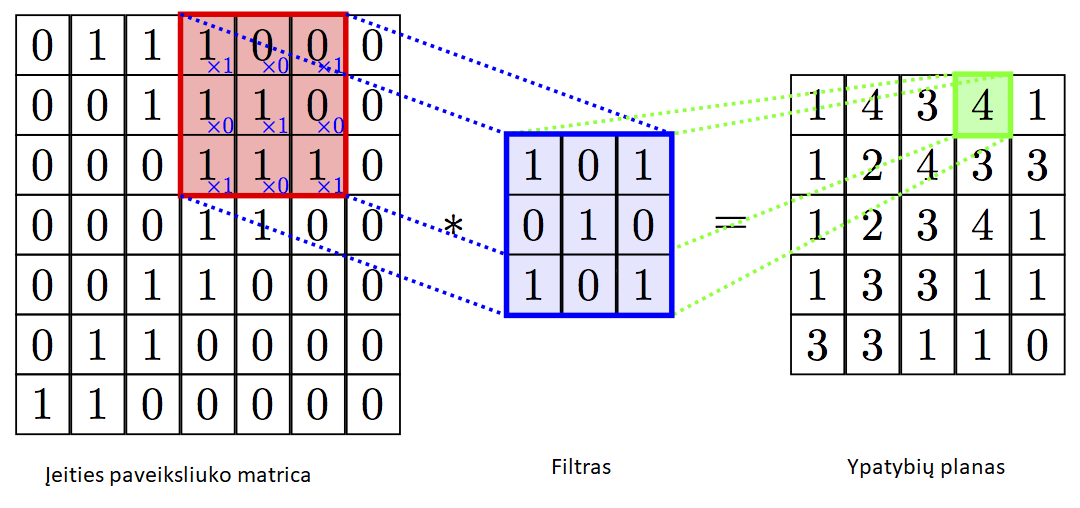
\includegraphics[width=0.5\textwidth]{img/Konvoliucija.png}
\caption{Konvoliucijos veikimas}
\end{figure}

Tačiau konvoliuciniai tinklai turi daug filtrų, kurie pereina per vieną paveiksliuką, kiekvienas išskirdamas skirtingą paveiksliuko ypatybę.
Pirmuose sluoksniuose šiuos filtrus galima įsivaizduoti kaip horizontalių, vertikalių ar įstrižų linijų filtrus, kurie sukuria paveikslėlio 
kraštų planą. Tinklas paima visus filtrus, gabaliukus paveiksliukų ypatybių vietų, ir juos sudeda į planą, kuris parodo ypatybės vietą. 
Mokydamasis skirtingų proporcijų ypatybių, tinklas leidžia lengvai kurti greitą ypatybių atpažinimą.

\subsection{Konvoliucinio neuroninio tinklo sluoksniai}
Konvoliuciniai neuroniniai tinklai tai yra sluoksnių rinkinys, kuris turi įeities, vidinius ir išeities sluoksnius. Tačiau priklausomai 
kokio tipo konvoliucinis neuroninis tinklas vidiniai sluoksniai gali skirtis. Konvoliuciniai neuroniniai tinklai turi tris pagrindinius 
sluoksnių tipus, kurie sudaro vidinį sluoksnį. Šie tipai yra konvoliucinis, sujungimo ir pilno sujungimo sluoksniai.

\subsubsection{Konvoliucinis sluoksnis}
Šis sluoksnis yra pagrindinis konvoliucinio neuroninio tinklo sluoksnis, kuris atlieka daugiausia skaičiavimų, nustato visas paveiksliuko ypatybes.
Kadangi, įeities informacija (paveiksliukas) yra didelės dimencijos neefektyvu visų neuronų sujungti vienus su kitais. Todėl neuronai yra sujungiami
su lokaliu informacijos kiekiu, kuris yra lygus filtro dydžiui ir vadinamas erdviniu mastu \cite{layers-CS231n}.

Neuronų kiekis po konvoliucijos (ypatybių plano dydis) yra nustatomas trimis parametrais:
\begin{itemize}
\item Gylis - atitinka filtrų skaičių.
\item Žingsnis - pikselių kiekis, kuris parodo per kiek reikia slinkti filtro matrica per įeities informacijos matricą.
\item Nulių pamušalas - įeities informacijos matrcios kraštus užpilduti nuliais.
\end{itemize}

\subsubsection{Sujungimo sluoksnis}
Periodiškai sujungimo sluoksnis yra įterpiamas tarp konvoliucinių. Pagrindinis sluoksnio tikslas yra laipsniškai mažinti erdvinį filtruojamo paveiskliuko mąstą.
Šis veikslas yra atliekams tam, kad sumažinti parametrų ir skaičiavimų kiekį bei kontroliuoti perjungimą. Sujungimo sluoksnis veikia nepriklausomai nuo kiekvieno
gabalėlio gylio ir keičia jo dydį erdviškai, naudodamas MAX operaciją. Dažniausiai šis sluoksnis yra naudojamas su 2x2 dydžio filtru - kas antras po konvoliucijos 
gauto gabaliuko kiekvienas gylio sluoksnis yra mažinamas per pusę ties ilgiu ir pločiu, taip yra atsikratoma 75 procentų aktyvacijų. Po šios operacijos gabaliuko 
gylis nepasikeičia.

Dažniausiai yra naudojamos dvi šio sluoksnio variacijos. Pirmasis yra vadinamas persidengiantis sujungimas, kur filtro dydis yra lygus 3 ir žingsnis yra lygus 2. 
O kitas dažniau naudojamas turi filtro dydį lygų 2 ir žingsnį taip pat 2. Sujungimo sluoksniai su labai dideliais parametrais yra labai desktruktyvūs.

\subsubsection{Pilno sujungimo sluoksnis}
Konvoliucinio ir sujungimo sluoksnių išeitys yra aukšto lygio ypatybės, kurios yra gautos iš įeities paveiksliuko. Pilno sujungimo sluoksnis yra sujungtas su visais 
neuronais iš sluoksnio buvusio prieš jį. Šio sluoksnio tikslas yra panaudojant tas ypatybes, kurios yra gautos iš prieš tai buvusių sluoksnių, nustatyti kokioms 
klasėms priklauso įeities paveiksliukas pagal mokymo informacijos rinkinį, kai nueroninio tinklo problema yra klasifikacija \cite{layers-fullyconnected}. Jei šiam sluoksniui yra naudojama 
minkštojo maksimumo funkcija tuomet sudėtis visų gautų galimybių turi būti lygi 1. Minkštojo maksimumo funkcija priima vektorių įvertinimų ir jį suspaudžia į 
vektorių, kuriame yra klasių tikimybių įvertinimai intervale nuo 0 iki 1, kur tikimybė arčiausiai vieneto reiškia, kad labiausiai užtikrintas dėl tos klasės.

\subsection{Architektūros}
Konvoliuciniai neuroniniai tinklai turi keletą skirtingų architektūrų, kurios yra naudojamos atinkmai pagal sprendžiamą problemą. 1 lentelėje pateikta infromaciją 
apie įvairias architektūras.


\begin{longtable}[h!]{ | p{4cm} | p{1cm} | p{3cm} | p{5cm} | p{2cm} | } 
\hline
Pavadinimas & Metai & Parametrų kiekis & Veikimas & ILSVRC vieta \\
\hline
LeNet & 1998 & 60 000 & Geriausiai atpažysta ranka paraštytus skaičius. Susideda iš sluoksnių - kelių pasikartojančių konvoliucijos ir sujungimo bei pasibaigia dviem pilno sujungimo sluoksniais. & - \\
\hline
AlexNet & 2012 & 60 000 000 & Veikimu panašus į LeNet, tačiau turi daug daugiau parametrų ir filtrų bei sudėtus konvoliucinius sluoksnius.  & pirma \\
\hline
GoogLeNet/Inception & 2014 & 4 000 000 & Vidiniai sluoksniai sudėti paraleliai, naudojami Inception moduliai. Vienas modulis savyje turi 1x1, 3x3 ir 5x5 dydžių konvoliucijos filtrų bei vidurkio sudėjimo sluoksnius. & pirma \\
\hline
VGGNet & 2014 & 138 000 000 & Panašus veikimas į AlexNet, tačiau daug gilesnis. Naudojamų filtrų dydis yra 3x3 ir jie yra sudėti vienas po kito. & antra \\
\hline
ResNet & 2015 & 25 000 000 & Turi labai daug sluoksnių, sudėtų vienas po kito, kurie turi liekamajį bloką, kuris įeities informaciją perduoda tolimesniam sluoksniui ją pridėdamas ir taip sumažina konvoliucijos ir aktyvavimo funkcijų kiekį.  & pirma \\
\hline
\caption{Konvoliucinių neuroninių tinklų architektūros}
\end{longtable}

\subsection{Modelio reguliavimas}
Pilnas konvoliucinio neuroninio tinklo apmokymas gali užtrukti labai ilgą laiką ir išnaudoti daug resursų. Todėl yra kai kurios įstaigos arba žmonės, kurie apmoko savo 
tinklą ir jo svorius bei reikšmes, vadinamą modeliu, pateikia visuomenei, tačiau šis modelis yra nepritaikytas individuoliai žmogaus užduočiai. Modelį reikia 
reguliuoti - iš naujo apmokyti paskutinius sluoksnius su individuolios užduoties parametrais.

Daugelis konvoliucinių neuroninių tinklų apmokytų su natūraliais paveiksliukais turi fenomeną. Pirmuosiuose sluoksniuose jie išmoksta ypatybių panašių į Gaboro filtą 
(tiesinis filtras naudojamas tekstūroms analizuoti) ir spalvų dėmes. Šios pirmojo sluoksnio ypatybės nepriklauso nuo duomenų rinkinio, bet yra bendros ir tinkamos 
daugeliui duomenų rinkinių ir užduočių \cite{DBLP:journals/corr/YosinskiCBL14}. Dėl šio fenomeno galima naudoti modelius neapmokytus su specifiniu duomenų rinkiniu, 
bet jį minimaliai modifiktą, kitoms užduotims spręsti, kas leidžia sutaupyti resursų bei turėti mažesnį duomenų rinkinį.

\section{Technologijos}
Naudojamų technologijų išsirinkimas yra pradinis žingsnis siekiant įvykdyti išsikeltas užduotis. Šiame skyriuje pateiktos populiariausios šių laikų technologijos 
bei trumpai papasakota apie jas.

\subsection{ImageNet}
ImageNet yra projektas sugalvotas profesorės Li Fei-Fei 2009 metais. Projekto tikslas buvo sukurti didelę sukategorizuotų paveiksliukų ir jų etikečių duomenų bazę, 
kuri butų skirta vizualinio objekto atpažinimo programinės įrangos tyrimams. Ši duomenų bazė yra suorganizuota pagal WorldNet hierarchija - anglų kalbos žodžiai 
yra grupuojami į sinonimų rinkinius, kurie turi apibūdinimus ir naudojimo pavyzdžius bei saugo ryšių kiekį tarp sinonimų arba jų narių. ImageNet turi daugiau nei 
100 000 sinonimų rinkinių, kur didžioji dalis yra daiktavardžiai (80 000+). 

Taip pat šis projektas kiekvienais metais daro konkursą vadinamą ,,ImageNet Large Scale Visual Recognition Challenge'' (trumpinys ILSVRC). Konkurso užduotis yra 
išmokinti modelį, kuris galėtų įeities paveiksliuką teisingai klasifikuoti į 1000 skirtingų objektų klasių, kurios atitinka realius daiktus, gyvūnus ir t.t. Modeliai 
yra apmokomi su apie 1.2 milijonų paveiksliukų ir dar 50 000 paveiksliukų yra naudojami validacijai mokymo metu bei 100 000 paveiksliukų yra panaudojami galutiniam 
modelio testavimui. Šis konkursas yra paveiksliukų klasifikacijos algoritmų etalonas.

\subsection{Keras}
Keras yra aukšto lygio programų sąsaja skirta neuroniniams tinklams. Sąsaja parašyta su ,,Python'' programavimo kalba ir vidinėje pusėje galinti veikti su ,,TensorFlow'' 
ir kitomis bibliotekomis. Keras buvo sukurtas tikintis suteikti greitą ekspermentavimą, kad sugalvojus idėją pasiekti rezultato būtų galima su kiek įmanoma mažiau uždėlsimo.

Ši sąsaja savyje turi visus pagrindinius neuroninio tinklo kūrimo blokus, pavyzdžiui, sluoskniai, aktyvavimo ir optimizavimo funkcijos. Taip pat Keras suteikia modelius, 
kurie yra apmokyti naudojant ImageNet duomenų bazę. Šiuos modelius galima reguliuoti, pridėti papildomų sluoksnių, pasirinkti esamus sluoksnius bei juos iš naujo apmokyti.

\subsection{TensorFlow}
TensorFlow yra atviros programinės įrangos biblioteka skirta aukšto našumo skaitinimas skaičiavimams. Jo lanksti architektūra leidžia lengvai diegti skaičiavimus įvairiose 
platformose - procesoriuose, grafikos procesoriuose. Sukurtas ,,Google'' dirbtinio intelekto skyriaus, tad yra labai palaikomas automatinis ir gilusis mokymasis, tačiau 
dėl bibliotekos ir skaičiavimų lankstumo yra naudojamas įvairiose mokslinėse srityse.

\section{Ekspermentas}
Šio ekspermento tikslas yra išanalizuoti mokymosi tikslumą su skirtingų gylių neuroninais tinklais, kai mokymui yra naudojamas mažas paveiksėlių rinkinys. Taigi, pirmas šio ekspermento žingsinis - išsirinkti konvoliucinį neuroninį tinklą. Poskyriuje ,,Architektūros'' yra trumpai apibūdinti pagrindiniai konvolicinių neuroninių tinklų tipai. Iš jų buvo išsirinktas VGG, kadangi jo veikimas ir sluoksnių išsidėstymas yra tinkamiausi išsikeltam tikslui įgyvendiniti. Buvo nuspręsta daryti paprastą, binarinę paveikslėlių klasifikaciją - nustatymas ar katė, ar šuo pavaizduotas paveikslėlyje.

\subsection{Duomenų rinkinys}
Šiais laikais konvoliuciniai neuroniniai tinklai pranoksta prieš tai buvusias naujausias technologijas naudotas paveiksliukų klasifikacijai. Viena iš pagrindinių priežasčių yra dideli ir gerai aprašyti duomenų rinkiniai, kaip kad ImageNet duomenų bazė. Geriausiai tinklas pasirodo, kai yra apmokomas su bendrinėm ypatybėm ir dar efektyviau pasirodo kai yra sureguliuoti su specifiniu duomenų rinkiniu \cite{http://adas.cvc.uab.es/task-cv2016/papers/0002.pdf}. Optimalus duomenų kiekis, kad gerai sureguliuoti modelį yra apie 10 000 paveiksliukų. 

Tačiau realybėje visų klasių objektų paveiksliukų nėra be galo daug, kadangi reikia skirti labai daug laiko ir žmogiškųjų resursų paveiksliukų žymėjimui bei turėti tiek daug paveiksliukų. Todėl tenka tinklus apmokyti su limituotais duomenų rinkiniais. Pagal šią realaus pasaulio problemą buvo įvykdyta viena iš ekspermento tikslo sąlygų - mažas duomenų rinkinys. Buvo surastas ir naudotas duomenų rinkinys, kuris turi 10 000 paveikslėlių - 8 000 mokymosi tikslui ir 2 000 validacijos.

\subsection{}


- CNN issirinkimas
- Duomenu radimas
CNN reguliavimo programos parasymas
bei programos pritaikymas modifikavimui
Skirtingu optimizavimo funkciju pritaikymas ir rezultatai


dataset:
8000 train
2000 validate

epoch - 40
trainbatch - 200
valbatch - 50

ft:
layers = 23
trainable = 8
total param - 40 406 849
trainable - 32 771 585
netrainable - 7 635 264

add lay:
layer = 34 
trainable = 19
total param - 51 952 449
trainable - 44 317 185
netrainable - 7 635 264

\sectionnonum{Rezultaitai ir išvados}
Darbo rezultatai:
\begin{itemize}
\item Pasirinktas tiriamas konvoliucinis neuroninis tinklas - VGG.
\item Rasta geriausia ir tinkamiausia optimizavimo funkicja - XX.
\item VGG buvo pritaikytas ir modifikuotas išsikeltam tikslui.
\item Konvoliucinis neuroninis tinklas buvo apmokytas.
\end{itemize}


Darbo išvados:
\begin{itemize}
\item 
\item
\end{itemize}

\printbibliography[heading=bibintoc] 

\end{document}
